\section{凸透镜的应用}\label{sec:1-8}

\xiaobiaoti{凸透镜成像的几种情况}
从上一节的实验,我们可以得到如图 \ref{fig:1-27} 所示的凸透镜成像的情况。

\begin{figure}[H]
    \centering
    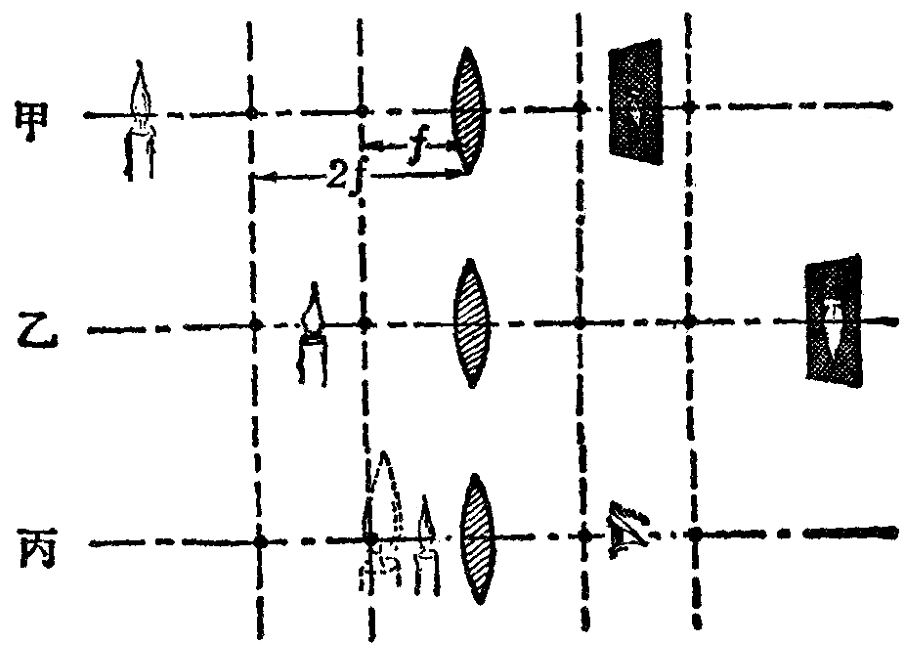
\includegraphics[width=0.6\textwidth]{../pic/czwl2-ch1-27}
    \caption{凸透镜成像}\label{fig:1-27}
\end{figure}

物体在凸透镜的焦点以外的时候,在透镜另一侧的光屏上总能得到倒立的实像,并且物距越小,像就越大,像距也越大。
当 $u > 2f$ 时,像是缩小的,$f < v < 2f$ (图 \ref{fig:1-27} 甲);
当 $2f > u > f$ 时,像是放大的,$v > 2f$(图 \ref{fig:1-27} 乙)。

物体在凸透镜的焦点以内的时候,在透镜的另一侧得不到物体的实像,
透过透镜可以看到正立、放大的像(图 \ref{fig:1-27} 丙)。
这个像跟平面镜成像相似,不是物体上各点发出的光实际会聚成的,所以是虚像。

\xiaobiaoti{照相机} 当 $u > 2f$ 时,凸透镜能够成缩小的实像,照相机就是利用这种现象来拍摄照片的。

\begin{figure}[htbp]
    \centering
    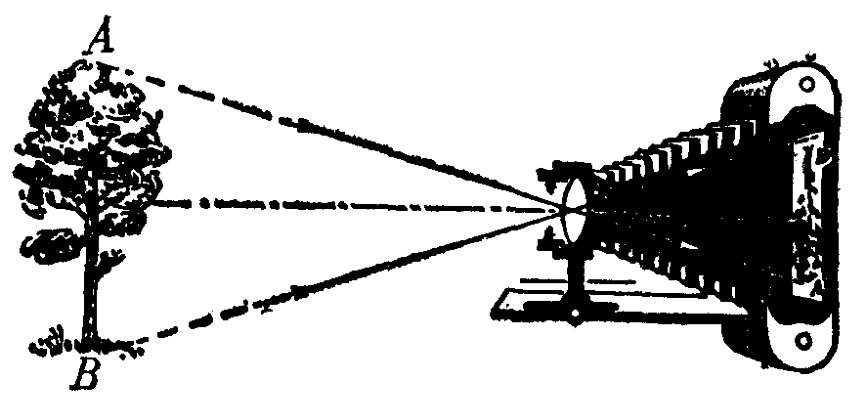
\includegraphics[width=0.6\textwidth]{../pic/czwl2-ch1-28}
    \caption{照相机示意图}\label{fig:1-28}
\end{figure}

照相机(图 \ref{fig:1-28})的前部有一个镜头,通常是由一组透镜组成的,它的作用相当于一个凸透镜。
镜头后面是暗箱,照相的感光胶片就装在暗箱的底部。选定了被照景物和照相的位置后,
调节暗箱的长度,也就是调节镜头的位置,使胶片上得到被照景物的清晰的倒立、缩小的实像。
胶片上的感光物质受到形成实像的光的照射,发生了化学变化,经过处理就得到底片,
然后由底片就可以得到照片。


\xiaobiaoti{幻灯机} 当 $2f > u > f$ 时,凸透镜能够成放大的实像,幻灯机就是利用这种现象,
把幻灯片上景物的像投射到银幕上的。

\begin{figure}[htbp]
    \centering
    \begin{minipage}{9cm}
    \centering
    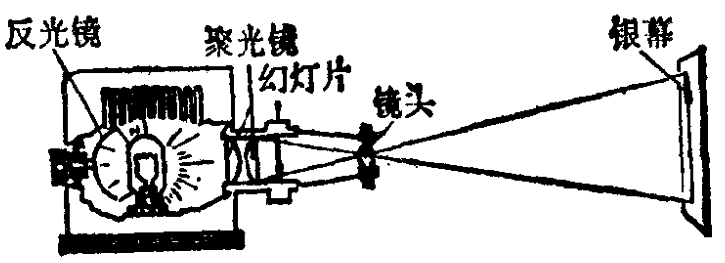
\includegraphics[width=8.5cm]{../pic/czwl2-ch1-29}
    \caption{幻灯机示意图}\label{fig:1-29}
    \end{minipage}
    \qquad
    \begin{minipage}{6cm}
    \centering
    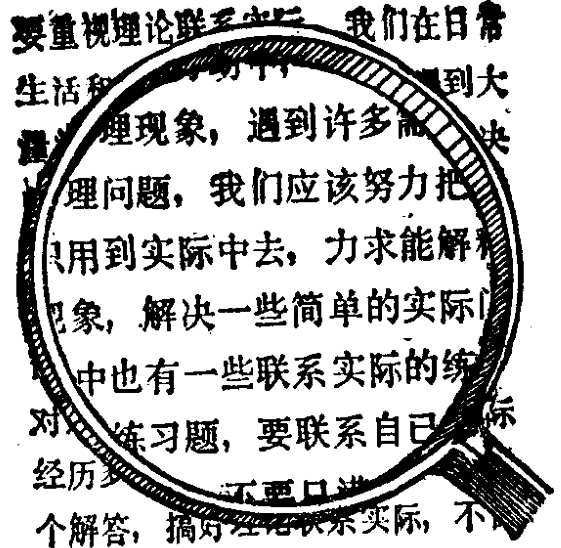
\includegraphics[width=4cm]{../pic/czwl2-ch1-30}
    \caption{放大镜}\label{fig:1-30}
    \end{minipage}
\end{figure}


图 \ref{fig:1-29} 是幻灯机的示意图。它前部的镜头相当于一个凸透镜,透明的幻灯片插在凸透镜后面比焦点略微远些的地方。
幻灯片后面是聚光镜,再后面是很强的光源和反光镜。光源发出的光和反光镜反射的光,经过聚光镜强烈地照亮幻灯片,
前后调整镜头的位置,银幕上就会出现幻灯片上景物的倒立、放大的实像。
我们要看到正立的像,只要把幻灯片倒过来插就行了。

\xiaobiaoti{放大镜} 当 $u < f$ 时,凸透镜能够成放大的虚像,放大镜就是利用这种现象来观察物体的。

使用放大镜的时候,必须把要观察的物体放在焦点以内才能看到正立、放大的虚像(图 \ref{fig:1-30})。



\section*{阅读材料:电影}

\begin{wrapfigure}[29]{r}{6.5cm}
    \centering
    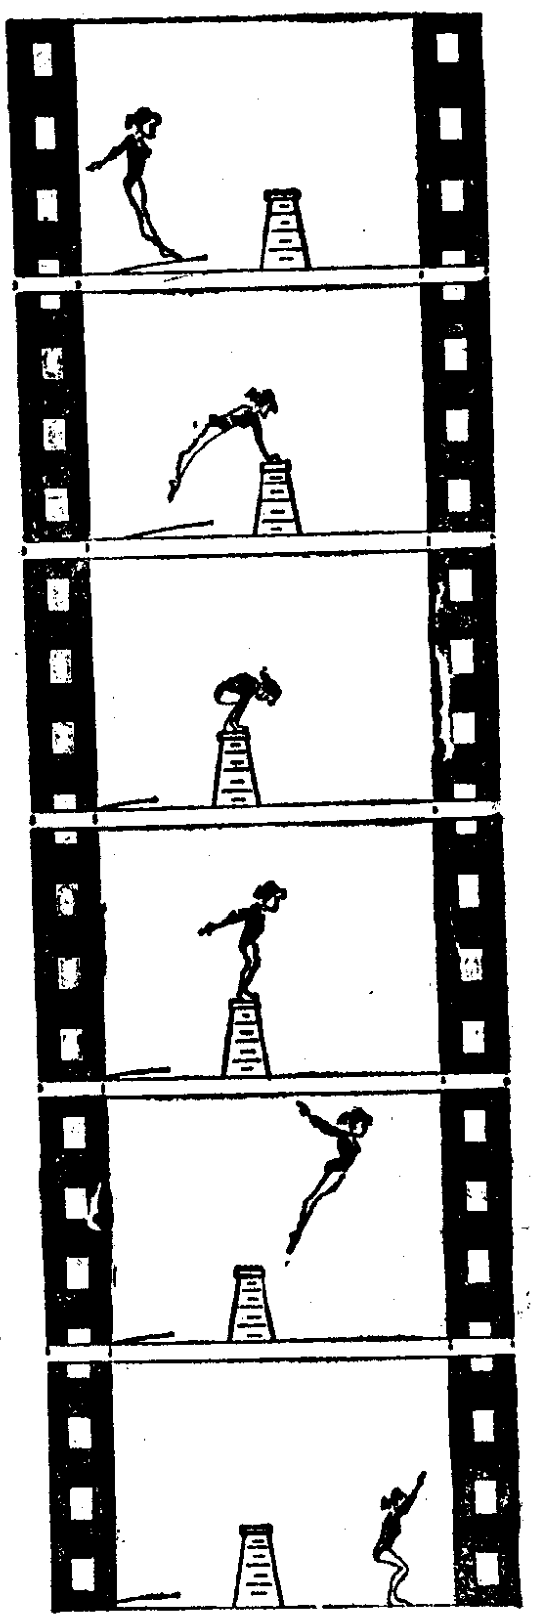
\includegraphics[width=5.5cm]{../pic/czwl2-ch1-31}
    \caption{电影片}\label{fig:1-31}
\end{wrapfigure}


电影放映机的构造相当复杂,但是它的投影原理跟幻灯机差不多,
也是利用相当于凸透镜的镜头把电影片上景物的像射到银幕上的。
不同的是,电影的画面是活动的。

\begin{enhancedline}
电影片上有一连串的照片。这些照片是对活动的景物每隔了 $\dfrac{1}{24}$ 秒拍一张拍摄下来的,
也就是说,一秒钟内要依次拍摄 24 张照片。因此,后一张跟前一张的景物的变化相差很小。
例如,拍摄体操运动员 6 ~ 7 秒钟内完的一个动作,在电影片上就留下了一百多张连续的照片。
图 \ref{fig:1-31} 是从这个过程中选出来的几个画面。
放映时,用电动机带动电影片,使它上面的照片依次从镜头后面通过,每秒钟通过 24 张。
每张照片都要在镜头后面停顿大约 0.04 秒的时间,它的放大的实像也在银幕上停留相同的时间。
在换照片的时候,电影放映机上有一个特殊的装置把镜头遮住,使银幕暂时黑暗。
但是我们看电影的时候,却觉得银幕上总有像,并且像中的景物是连续活动的,这是为什么呢?
\end{enhancedline}

这是因为人的视觉有一种叫做视觉暂留的特性,就是外界的景物消失以后,视神经对它的印象还会保留 0.1 秒的时间。
在黑暗中,迅速地移动一支点燃着的香,会看到香的亮点变成了一条亮线,就是由于视觉暂留。
放电影时,银幕上相继出现的像相隔的时间(也就是银幕黑暗的时间)不到 0.01 秒,并且它们上面的景物变化很小,
由于视觉暂留的缘故,我们就觉得像是连续活动的了。

通常,我们看的电影,银幕上的景物活动的情况跟实际上的快慢程度是一致的。
这是因为拍摄电影跟放映电影的速度相同,即拍摄时每秒拍 24 张,放映时也是每秒放 24 张。
如果拍摄时加快拍摄速度,例如每秒拍 3900 张,而放映时仍每秒放 24 张,那么银幕上的动作就会比实际的慢一百六十多倍。
实际的动作在电影里就是慢悠悠的了。这就是电影里的慢镜头。
相反,如果放慢拍摄速度,而按正常速度放映,结果银幕上的动作就会比实际的快。
实际的动作是很缓慢的,在电影里却是刹那间完成了。这就是电影里的快镜头。

电影的快、慢镜头,不但在一般的电影里被用来达到一定的艺术效果,在科学研究上也很重要。
例如,使用慢镜头可以更仔细地观察一个物体的运动。

电影不但丰富了我们的文化生活,而且能能够把各种活动情况有声有色地记录下来。
因此,电影是一种很好的记录工具。



\lianxi

(1) 有经验的渔民在叉鱼的时候,不把叉对准所看到的鱼的位置,而是对着稍低于所看到的鱼的位置叉去,才能叉到鱼。为什么?

(2) 图 \ref{fig:1-32} 中画出了光通过透镜前后的方向,在图中填上适当类型的透镜。

\begin{figure}[htbp]
    \centering
    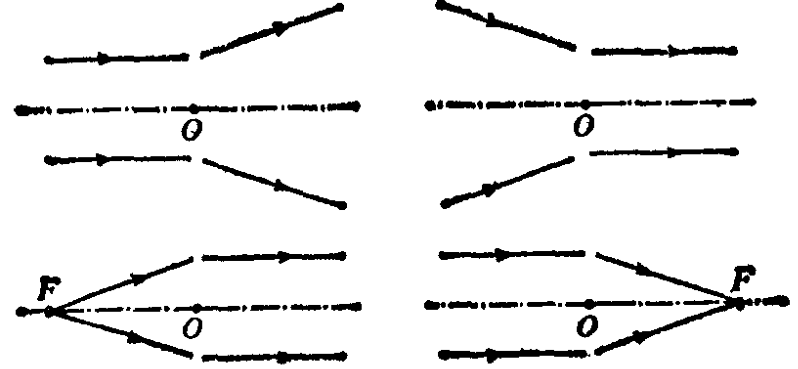
\includegraphics[width=0.6\textwidth]{../pic/czwl2-ch1-32}
    \caption{}\label{fig:1-32}
\end{figure}

(3) 有两个凸透镜,要想使一束跟它们的主轴平行的光通过它们后仍平行射出,这两个凸透镜应当怎样放置?
画出这一束光通过这两个凸透镜的情况。

(4) 用镜头焦距一定的照相机照相,想使照片上的人像大一些,照相机应该离被照的人近一些,还是远一些?

(5) 放映幻灯的时候,想使银幕上的像大一些,应该使幻灯机离银幕近一些,还是远一些?

